\documentclass[12pt, a4paper]{article}
\usepackage[margin=1in]{geometry}
\usepackage[latin1]{inputenc}
\usepackage{titlesec}
\usepackage{amsmath}
\usepackage{amsthm}
\usepackage{amsfonts}
\usepackage{amssymb}
\usepackage{array}
\usepackage{booktabs}
\usepackage{ragged2e}
\usepackage{enumerate}
\usepackage{enumitem}
\usepackage{cleveref}
\usepackage{slashed}
\usepackage{commath}
\usepackage{lipsum}
\usepackage{colonequals}
\usepackage{addfont}
\addfont{OT1}{rsfs10}{\rsfs}
\renewcommand{\baselinestretch}{1.1}
\usepackage[mathscr]{euscript}
\let\euscr\mathscr \let\mathscr\relax
\usepackage[scr]{rsfso}
\newcommand{\powerset}{\raisebox{.15\baselineskip}{\Large\ensuremath{\wp}}}
\usepackage{longtable}
\usepackage{multirow}
\usepackage{multicol}
\usepackage{calligra}
\usepackage[T1]{fontenc}
\newcounter{proofc}
\renewcommand\theproofc{(\arabic{proofc})}
\DeclareRobustCommand\stepproofc{\refstepcounter{proofc}\theproofc}
\newenvironment{twoproof}{\tabular{@{\stepproofc}c|l}}{\endtabular}
\newcolumntype{C}{>$c<$}
\usepackage{fancyhdr}
\pagestyle{fancy}
\fancyhf{}
\renewcommand{\headrulewidth}{0pt}
\fancyhead[R]{\thepage}
\usepackage{enumitem}
\usepackage{tikz}
\usepackage{commath}
\usepackage{colonequals}
\usepackage{bm}
\usepackage{tikz-cd}
\renewcommand{\baselinestretch}{1.1}
\usepackage[mathscr]{euscript}
\let\euscr\mathscr \let\mathscr\relax
\usepackage[scr]{rsfso}
\usepackage{titlesec}
\graphicspath{{./Ramsey Theory/}}
\newcommand*{\logeq}{\ratio\Leftrightarrow}
  
\setlist[description]{leftmargin=6mm,labelindent=4mm}
  
\begin{document}

\justifying

\section{Overview}

Broadly speaking, the goal of the program to be discussed throughout this paper is to aid in the research of what is called \textit{Pseudo Ramsey Theory} (PRT). The objects of interest in PRT are what are called \textit{colorings}, and \textit{pseudo progressions}. Specifically, PRT aims to use tools from combinitorics to count these objects, or at least determine upper and lower bounds for the count. \par

\vspace{6mm}

\noindent\textit{\textbf{Terminology}}

\vspace{2mm}
Given a number $n\in\mathbb{N}$, we wish to color each number 1 2 3 $\dots$ $n$ one of $r\in\mathbb{N}$ many colors. By the multiplication principle, there are $r^n$ many ways to do this, and so we would say that there are $r^n$ many colorings of $[n]$, where $[n]=\{1,\dots,n\}$. Now that we have all of our $r^n$ colorings in our mind, we then wish to know if it is true that \underline{every} one of these colorings contains a \textit{monochromatic} $k$-\textit{length} $m$-\textit{pseudo progression}.\par
The definition of the last term is as follows: Given some $n\in\mathbb{N}$, the number $k\leq n$ will denote the length of, or number of terms in, a progression of numbers $a_1,a_2,\dots,a_k\in[n]$, where $a_i<a_{i+1}$, for $1\leq i\leq k$. Now suppose we have a set $D\subset\mathbb{N}$, where $\abs{D}=m$ and $m\leq k-1$. This set denotes the set of \textit{common differences}. The elements of this set represent the differences between every pair of consecutive terms in the given progression. So we have that for $a_{i+1}-a_i\in D$, for $1\leq i< k$. With all the previous items in place, we would call the progression $a_1,a_2,\dots,a_k$ a $k$-\textit{length} $m$-\textit{pseudo progression}.\par

\vspace{6mm}

\noindent\textit{\textbf{Example 1.1}}

\vspace{2mm}
Consider the following example. Let $n=10$ and $k=4$. Then if we wanted to know what type of pseudo progression 2,3,7,8 is, we would look at the differences between each consecutive pair of numbers. Thus, we have that $3-2=1$, $7-3=4$, and $8-7=1$. This means that, for this particular progression, we have that $a_{i+1}-a_i\in\{1,4\}$ for $1\leq i<4$. Since $\abs{\{1,4\}}=2$, we would classify 2,3,7,8 as a $2$-pseudo progression. It should be noted that it would be completely true if we stated that $a_{i+1}-a_i\in\{1,2,4\}$ for $1\leq i<4$. The reason we can say this is because $\{1,4\}\subset\{1,2,4\}$ and so any element of $\{1,4\}$ is an element of $\{1,2,4\}$. More importantly however, is that this means 2,3,7,8 is a 3-pseudo progression since all of its differences are contained in the set $\{1,2,4\}$ and $\abs{\{1,2,4\}}=3$. In other words, the set of 2-pseudo progressions is a subset of the set of 3-pseudo progressions. Similarly, the set of 1-pseudo progressions (arithmetic progressions) is a subset of the set of 2-pseudo progressions.

\vspace{6mm}

\noindent\textit{\textbf{Conclusion}}

\vspace{2mm}

The last thing we need to define is the term \textit{monochromatic}. So at this point we know that given some $n,r\in\mathbb{N}$, where $r$ denotes the number of colors, there are $r^n$ many ways to color the progression $1,\dots,n$. Additionally, given some $k,m\in\mathbb{N}$, we can determine (both through the a proven formula and the program) how many $k$-length $m$-pseudo progressions can be formed from the terms in $[n]$. For now, we will denote this number as $s$. So supposing that we have $s$ many $k$-length $m$-pseudo progressions, we want to know if in every one of the $r^n$ colorings of $1,\dots,n$, we can find a $k$-length $m$-pseudo progression where all of its terms are of one color, i.e., \textit{monochromatic}.

\section{The Program}

To explain how this program works we will look at each of its parts independently. The core of the program is based on the following approach to the PRT problem. Suppose we are given $n,k,m,r\in\mathbb{N}$. Now assume that there are $s$ many $k$-length $m$-pseudo progressions. Moreover, we know that there are $r^n$ possible colorings of $1,\dots,n$. So of these $r^n$ many colorings, how many of them contain a monochromatic $k$-length $m$-pseudo progression?\par
To answer this we first will consider 1 of the $s$ many $k$-length $m$-pseudo progressions we have available. Let $a_1,\dots,a_k$ be one of these progressions. Since this progression has $k$ many terms, then there are $n-k$ many numbers not present in this progression. So suppose we color this progression red and ask how many of the $r^n$ possible colorings contains a red version of $a_1,\dots,a_k$. Since there are $n-k$ many terms not present in this progression, then this means that each of the $n-k$ terms can be any one of the $r$ colors. Thus, by the multiplication principle, there should be $r^{n-k}$ many colorings which contain a red version of the progression $a_1,\dots,a_k$. \par
It follows that the same should apply to the remaining $s-1$ progressions and so there should be $sr^{n-k}$ many colorings which contain a red $k$-length $m$-pseudo progression. Lastly, since our choice to color these progressions red was arbitrary and we could have colored them any one of the $r$ many colors, then this implies that there are $rsr^{n-k}=sr^{n-k+1}$ many colorings that contain a monochromatic $k$-length $m$-pseudo progression.

\vspace{6mm}

\noindent\textbf{DEFINITION: } Given $n,k,m,r\in\mathbb{N}$, the \textit{\textbf{approximate span}} of the $s$ many $k$-length $m$-pseudo progressions is defined as $AS(n,k,m,r)=sr^{n-k+1}$.

\vspace{6mm}

As we will see in the following example, the approximate span is an over count of colorings. This means we will need a way to determine the over count factor and subtract it off from the approximate span.

\vspace{6mm}

\noindent\textit{\textbf{Example 2.1}}

\vspace{2mm}

Let $n=5, k=3, m=1,$ and $r=3$. With these given values there are $4$ 3-length 1-pseudo progressions. Namely,

\begin{equation*}
    \begin{split}
        &1,2,3 \\
        &1,3,5 \\
        &2,3,4 \\
        &3,4,5.
    \end{split}
\end{equation*}



\begin{figure}
    \hspace{10mm}
    \includegraphics{"1PR".png}
    \caption{3 Coloring of 3-length Arithmetic Progressions}
    \label{fig:my_label}
\end{figure}

\noindent Now suppose we colored each of these progressions red. Above is a matrix-type representation of all of the colorings that contain one of the given red progressions. The first thing that stands out is the top row of each matrix is identical. We can also see that row 2 of matrix $A$ is identical to row 2 of matrix $D$, and so on. This shows us that in the $sr^{n-k}=36$ colorings in the above figure, there are repeated rows.So how do we determine the over count factor?\par
Suppose we let $0:=$red, $1:=$blue, and $2:=$yellow. Then the fifth row of matrix $A$, for instance, can be written as 

\vspace{4mm}

\begin{center}
    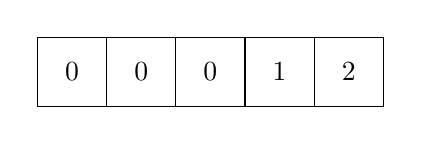
\begin{tikzpicture}
        \matrix [matrix of nodes, style={nodes={rectangle,draw,minimum width=2.5em}}, minimum height=2.5em, row sep=-\pgflinewidth, column sep=-\pgflinewidth]
            {
                0 & 0 & 0 & 1 & 2\\
            };
    \end{tikzpicture}.
\end{center}

\noindent Now suppose that we took the column indices of this row and sent them to a function, call it $P(j)$, that returns the $j^{\text{th}}$ prime number. So then we have that 

\begin{equation*}
    \begin{split}
        P(1) &= 2 \\
        P(2) &= 3 \\
        P(3) &= 5 \\
        P(4) &= 7 \\
        P(5) &= 11 \\
        &\vdots
    \end{split}
\end{equation*}

Next, for each $P(j)$, we will raise it to the power equal to the value stored in the $j^{\text{th}}$ column and take the product of the resulting powers of primes and assign this number to that row. Thus,

\begin{equation*}
    \begin{split}
        A_5 &: \prod\limits_{j=1}^{5}P(j)^{A_{5j}} \\
        &= P(1)^{A_{51}}P(2)^{A_{52}}P(3)^{A_{53}}P(4)^{A_{54}}P(5)^{A_{55}} \\
        &= 2^03^05^07^111^2 \\
        &=847.
    \end{split}
\end{equation*}

\noindent So what we have done is assigned a unique number to the row 5 of matrix $A$. If we did this for each row for each matrix, the resulting list of numbers would be

\begin{align*}
        A_1 & : 1 & B_1 & : 1 & C_1 & : 1 & D__1 & : 1 \\
        A_2 & : 11 & B_2 & : 7 & C_2 & : 11 & D_2 & : 3\\ 
        A_3 & : 7 & B_3 & : 3 & C_3 & : 2& D_3 & : 2\\ 
        A_4 & : 77 & B_4 & : 21 & C_4 & : 22& D_4 & : 6\\
        A_5 & : 847 & B_5 & : 147& C_5 & : 242& D_5 & : 18\\ 
        A_6 & : 539& B_6 & : 63& C_6 & : 44& D_6 & : 12\\ 
        A_7 & : 5929& B_7 & :441 & C_7 & : 484& D_7 & : 36 \\ 
        A_8 & : 49& B_8 & : 9 & C_8 & : 4& D_8 & : 4 \\ 
        A_9 & : 121& B_9 & : 49 & C_9 & :121 & D_9 & : 9 \\ 
\end{align*}

\noindent Now suppose we place all of these numbers into one list. We will then start at the number assigned to $A_1$ and compare it to every other number in the list. If the comparison yields an equality, then we will add 1 to a counter and remove the identical item from the list.\par A rough flow chart of this might look like

\begin{equation*}
    \begin{split}
        A_1 &\neq A_2 \rightarrow c = 0 \\
        A_1 &\neq A_3 \rightarrow c = 0 \\
        &\vdots \\
        A_1 &= B_1\rightarrow c = 1 \\
        &\vdots \\
        A_1 &= C_1\rightarrow c=2 \\
        &\vdots \\
        A_1 &= D_1\rightarrow c = 3 \\
        &\vdots
    \end{split}
\end{equation*}

\newpage

After doing this comparison with $A_1$, $c=3$ and the resulting list would be

\begin{align*}
        A_1 & : 1 &  &  &  &  &  & \\
        A_2 & : 11 & B_2 & : 7 & C_2 & : 11 & D_2 & : 3\\ 
        A_3 & : 7 & B_3 & : 3 & C_3 & : 2& D_3 & : 2\\ 
        A_4 & : 77 & B_4 & : 21 & C_4 & : 22& D_4 & : 6\\
        A_5 & : 847 & B_5 & : 147& C_5 & : 242& D_5 & : 18\\ 
        A_6 & : 539& B_6 & : 63& C_6 & : 44& D_6 & : 12\\ 
        A_7 & : 5929& B_7 & :441 & C_7 & : 484& D_7 & : 36 \\ 
        A_8 & : 49& B_8 & : 9 & C_8 & : 4& D_8 & : 4 \\ 
        A_9 & : 121& B_9 & : 49 & C_9 & :121 & D_9 & : 9. \\ 
\end{align*}

Running the procedure again but with $A_2$, we would have $c=4$ and

\begin{align*}
        A_1 & : 1 &  &  &  &  &  & \\
        A_2 & : 11 & B_2 & : 7 &  &  & D_2 & : 3\\ 
        A_3 & : 7 & B_3 & : 3 & C_3 & : 2& D_3 & : 2\\ 
        A_4 & : 77 & B_4 & : 21 & C_4 & : 22& D_4 & : 6\\
        A_5 & : 847 & B_5 & : 147& C_5 & : 242& D_5 & : 18\\ 
        A_6 & : 539& B_6 & : 63& C_6 & : 44& D_6 & : 12\\ 
        A_7 & : 5929& B_7 & :441 & C_7 & : 484& D_7 & : 36 \\ 
        A_8 & : 49& B_8 & : 9 & C_8 & : 4& D_8 & : 4 \\ 
        A_9 & : 121& B_9 & : 49 & C_9 & :121 & D_9 & : 9. \\ 
\end{align*}

Then with $A_3$ we have $c=5$ and

\begin{align*}
        A_1 & : 1 &  &  &  &  &  & \\
        A_2 & : 11 &  &  &  &  & D_2 & : 3\\ 
        A_3 & : 7 & B_3 & : 3 & C_3 & : 2& D_3 & : 2\\ 
        A_4 & : 77 & B_4 & : 21 & C_4 & : 22& D_4 & : 6\\
        A_5 & : 847 & B_5 & : 147& C_5 & : 242& D_5 & : 18\\ 
        A_6 & : 539& B_6 & : 63& C_6 & : 44& D_6 & : 12\\ 
        A_7 & : 5929& B_7 & :441 & C_7 & : 484& D_7 & : 36 \\ 
        A_8 & : 49& B_8 & : 9 & C_8 & : 4& D_8 & : 4 \\ 
        A_9 & : 121& B_9 & : 49 & C_9 & :121 & D_9 & : 9. \\ 
\end{align*}

\newpage

Then with $A_4-A_7$ we find that those numbers do not repeat and thus nothing changes. So then after doing the comparison with $A_8$ we get $c=6$ and

\begin{align*}
        A_1 & : 1 &  &  &  &  &  & \\
        A_2 & : 11 &  &  &  &  & D_2 & : 3\\ 
        A_3 & : 7 & B_3 & : 3 & C_3 & : 2& D_3 & : 2\\ 
        A_4 & : 77 & B_4 & : 21 & C_4 & : 22& D_4 & : 6\\
        A_5 & : 847 & B_5 & : 147& C_5 & : 242& D_5 & : 18\\ 
        A_6 & : 539& B_6 & : 63& C_6 & : 44& D_6 & : 12\\ 
        A_7 & : 5929& B_7 & :441 & C_7 & : 484& D_7 & : 36 \\ 
        A_8 & : 49& B_8 & : 9 & C_8 & : 4& D_8 & : 4 \\ 
        A_9 & : 121& & & C_9 & :121 & D_9 & : 9. \\ 
\end{align*}

\noindent And then with $A_9$ we get $c=7$ and

\begin{align*}
        A_1 & : 1 &  &  &  &  &  & \\
        A_2 & : 11 &  &  &  &  & D_2 & : 3\\ 
        A_3 & : 7 & B_3 & : 3 & C_3 & : 2& D_3 & : 2\\ 
        A_4 & : 77 & B_4 & : 21 & C_4 & : 22& D_4 & : 6\\
        A_5 & : 847 & B_5 & : 147& C_5 & : 242& D_5 & : 18\\ 
        A_6 & : 539& B_6 & : 63& C_6 & : 44& D_6 & : 12\\ 
        A_7 & : 5929& B_7 & :441 & C_7 & : 484& D_7 & : 36 \\ 
        A_8 & : 49& B_8 & : 9 & C_8 & : 4& D_8 & : 4 \\ 
        A_9 & : 121& & & & & D_9 & : 9. \\ 
\end{align*}

\noindent Now we move on to $B_3$. This yields $c=8$ and 

\begin{align*}
        A_1 & : 1 &  &  &  &  &  & \\
        A_2 & : 11 &  &  &  &  &  & \\ 
        A_3 & : 7 & B_3 & : 3 & C_3 & : 2& D_3 & : 2\\ 
        A_4 & : 77 & B_4 & : 21 & C_4 & : 22& D_4 & : 6\\
        A_5 & : 847 & B_5 & : 147& C_5 & : 242& D_5 & : 18\\ 
        A_6 & : 539& B_6 & : 63& C_6 & : 44& D_6 & : 12\\ 
        A_7 & : 5929& B_7 & :441 & C_7 & : 484& D_7 & : 36 \\ 
        A_8 & : 49& B_8 & : 9 & C_8 & : 4& D_8 & : 4 \\ 
        A_9 & : 121& & & & & D_9 & : 9. \\ 
\end{align*}

\newpage

\noindent We find that the numbers assigned to $B_4-B_7$ do not repeat and so moving on to $B_8$ we get $c=9$ and 

\begin{align*}
        A_1 & : 1 &  &  &  &  &  & \\
        A_2 & : 11 &  &  &  &  &  & \\ 
        A_3 & : 7 & B_3 & : 3 & C_3 & : 2& D_3 & : 2\\ 
        A_4 & : 77 & B_4 & : 21 & C_4 & : 22& D_4 & : 6\\
        A_5 & : 847 & B_5 & : 147& C_5 & : 242& D_5 & : 18\\ 
        A_6 & : 539& B_6 & : 63& C_6 & : 44& D_6 & : 12\\ 
        A_7 & : 5929& B_7 & :441 & C_7 & : 484& D_7 & : 36 \\ 
        A_8 & : 49& B_8 & : 9 & C_8 & : 4& D_8 & : 4 \\ 
        A_9 & : 121& & & & &  & . \\ 
\end{align*}

\noindent And now on to $C_3$. This yields $c=10$ and 

\begin{align*}
        A_1 & : 1 &  &  &  &  &  & \\
        A_2 & : 11 &  &  &  &  &  & \\ 
        A_3 & : 7 & B_3 & : 3 & C_3 & : 2&  & \\ 
        A_4 & : 77 & B_4 & : 21 & C_4 & : 22& D_4 & : 6\\
        A_5 & : 847 & B_5 & : 147& C_5 & : 242& D_5 & : 18\\ 
        A_6 & : 539& B_6 & : 63& C_6 & : 44& D_6 & : 12\\ 
        A_7 & : 5929& B_7 & :441 & C_7 & : 484& D_7 & : 36 \\ 
        A_8 & : 49& B_8 & : 9 & C_8 & : 4& D_8 & : 4 \\ 
        A_9 & : 121& & & & &  & . \\ 
\end{align*}

\newpage

\noindent The numbers assigned to $C_4-C_7$ do not repeat and so after doing the comparison with $C_8$, we get $c=11$ and 

\begin{align*}
        A_1 & : 1 &  &  &  &  &  & \\
        A_2 & : 11 &  &  &  &  &  & \\ 
        A_3 & : 7 & B_3 & : 3 & C_3 & : 2&  & \\ 
        A_4 & : 77 & B_4 & : 21 & C_4 & : 22& D_4 & : 6\\
        A_5 & : 847 & B_5 & : 147& C_5 & : 242& D_5 & : 18\\ 
        A_6 & : 539& B_6 & : 63& C_6 & : 44& D_6 & : 12\\ 
        A_7 & : 5929& B_7 & :441 & C_7 & : 484& D_7 & : 36 \\ 
        A_8 & : 49& B_8 & : 9 & C_8 & : 4&  &  \\ 
        A_9 & : 121& & & & &  & . \\ 
\end{align*}

\noindent Lastly, none of the numbers assigned to $D_4-D_8$ repeat and the whole procedure concludes with $c=11$. Now if we take our initial count of $36$ colorings which contained a red version of the desired pseudo progressions and subtract from it the value $c=11$, we get $25$. This number represents the total number of distinct colorings which contain a red monochromatic 3-length 1-pseudo progression. \par
As discussed earlier, the choice of red was arbitrary and so we can perform the same processing all over again with blue or yellow and we would get 25 each time. Thus, the total span, or just span, of our 4 pseudo progressions is $r(sr^{n-k}-c)=3(4\cdot3^2-11)=75$. Thus, for $n=5, k=3,m=1$, and $r=3$, there are 75 colorings of $1,2,3,4,5$ which contain a monochromatic 3-length 1-pseudo progression. However, since there are $r^n=3^5=243$ possible colorings, then $243-75=168$ colorings do not contain a monochromatic 3-length 1-pseudo progression. Therefore, it is not true that \textit{every} coloring of 1,2,3,4,5, given 3 colors, contains a monochromatic 3-length 1-pseudo progression.

\vspace{6mm}

\noindent\textbf{DEFINITION: } Given $n,k,m,r\in\mathbb{N}$ and assuming there are $s$ many $k$-length $m$-pseudo progressions, then if the over count factor in the approximate span is equal to $c$, then the \textit{\textbf{span}} of those pseudo progressions is equal to $r(s\cdot r^{n-k}-c)=span(n,k,r,m)$.

\vspace{6mm}

\textit{\textbf{Lemma. }}\textit{Given $n,k,m,r,s,c\in\mathbb{N}$, where $s$ is the number of $k$-length $m$-pseudo progressions and $c$ is the number of repeated colorings in the approximate span of the $s$ pseudo progressions, then if $span(n,k,r,m)=r^n$, then every coloring of $1,\dots,n$ contains a monochromatic $k$-length $m$-pseudo progression.}

\newpage

\begin{description}
    \item$(5,3,1,2)$: FALSE
    \item$(5,3,1,3)$: FALSE
    \item$(5,3,2,2)$: TRUE
    \item$(5,4,1,2)$: FALSE
    \item$(5,4,2,2)$: FALSE
    \item$(5,4,2,3)$: FALSE
    \item$(6,3,1,2)$: FALSE
    \item$(6,3,2,2)$: TRUE
    \item$(6,3,2,3)$: FALSE
    \item$(6,4,1,2)$: FALSE
    \item$(6,4,2,2)$: FALSE
    \item$(6,4,2,3)$: FALSE
    \item$(6,4,3,2)$: FALSE
    \item$(6,4,3,3)$: FALSE
    \item$(7,3,1,2)$: FALSE
    \item$(7,3,1,3)$: FALSE
    \item$(7,3,2,2)$: TRUE
    \item$(7,3,2,3)$: TRUE
    \item$(7,4,1,2)$: FALSE
    \item$(7,4,1,3)$: FALSE
    \item$(7,4,2,2)$: FALSE
    \item$(7,4,2,3)$: FALSE 
    \item$(7,4,3,2)$: TRUE
    \item$(7,4,3,3)$: FALSE
    \item$(8,3,1,2)$: TRUE
    \item$(8,3,1,3)$: 
    \item$(8,4,2,2)$: TRUE
    \item$(8,5,2,2)$: FALSE
    \item$(8,4,3,2)$: TRUE
    \item$(8,4,3,3)$: FALSE
    \item$(8,5,2,2)$: FALSE
    \item$(8,5,3,2)$: FALSE
    \item$(8,5,4,2)$: FALSE
    \item$(8,6,2,2)$: FALSE
\end{description}


  
\end{document}